\documentclass[a4paper, 11pt, twocolumn]{article}
\usepackage[margin=0.8in]{geometry}
\usepackage{xcolor}
\usepackage{graphicx} %package to manage images
\graphicspath{ {./images/} }

\title{Instrumentation Systems\footnote{Images from Wjec E-book}}
\author{Revision sheet}
\date{}

\begin{document}
    
    \maketitle
    \section{Analogue Instrumentation}
    There are two key types of analogue instrumentation systems:
    \begin{itemize}
        \item Potential divider circuit
        \item Wheatstone bridge.
    \end{itemize}
    \subsection{Potential divider circuit}
    For example, this is a temperature sensing subsystem.\\
    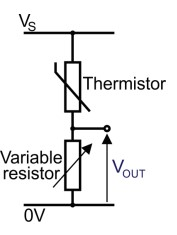
\includegraphics{simplePD.jpg} \\
    There are a number of issues with the potential divider circuit, all of which can be overcome by using a Wheatstone bridge.
    \begin{itemize}
        \item Affected by supply voltage fluctustions
        \item Resistance is affected by factors other than intended (eg, humidity)
    \end{itemize}

    \subsection{Wheatstone bridge}
    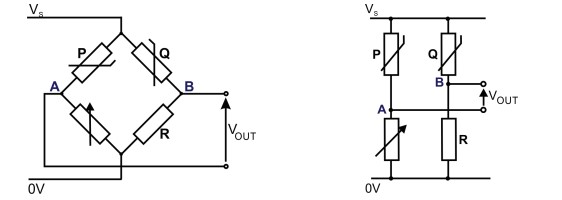
\includegraphics[width=8cm]{wheatstoneBridge.jpg} \\
    Both diagrams are of the same circuit, however the one on the right is easier to understand.
    The fundamentals of this circuit can be defined in the following equation: \\
    If $\frac{P}{VR}=\frac{Q}{R} $ (ratio of resisotrs is the same on both sides of the bridge)\\
    $V_P = V_Q$\\
    $Vout = 0V$ (This means the bridge is balanced, which is what we want!) \\
    If $V_S$ increases, $V_Q$ and $V_P$ both increase proportionally therefore the bridge stays balanced.
    Both P and Q are subjected to the same environment, however only Q is attached to the temperature being measured. This compensates against voltage changes due to unwanted environmental changes.
    \subsection{Measure-y things}
    \begin{itemize}
        \item Thermistor
        \item Light Dependant resisotrs
        \item Strain gauge
    \end{itemize}
    \subsection{Instrumentation amplifier}
    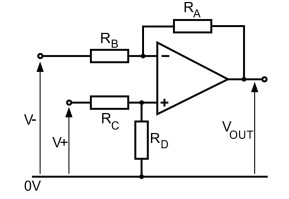
\includegraphics{instrumentationAmp.jpg} \\
    The output from the Wheatstone bridge is tiny, we have to amplify it. The amplifier has to have a high CMRR and a high input impedance. \\
    $R_F = R_D$\\
    $R_1 = R_2$\\
    $Vout = (V_+ - V_-)\times\frac{R_F}{R_1}$ \\

    \section{Digital Instrumentation}
    The simplest form of input is a button. \\
    Digital inputs can either be on (1) or off (0).
    \subsection{Slotted Disc}
    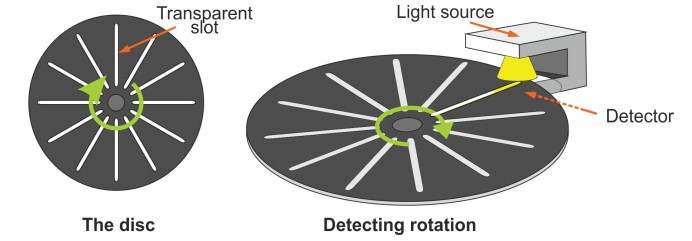
\includegraphics[width=8cm]{slottedDisk.jpg} \\
    The disc spins around inside a reader where a beam of light is shone through and where there is a slot in the disc, it hits the detector. The light is quite often infra-red light. It is only useful to measure speed/number of rotations as it doesn't show direction.
    \subsection{Encoded disc}
    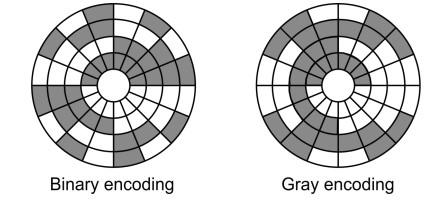
\includegraphics[width=8cm]{encodedDisk.jpg} \\
    The position is measured using opto-switches which shine a light down to the disc and record the reflection which comes back from it.
    \subsubsection{Binary encoded disc}
    This is better than a slotted disc as each sector tells us exactly which part of the disc it is on therefore we can measure absolute position.
    There are still problems with this disc: when the disc advances from 000 to 111, it isn't registerd cleanly there are intermediary false readings which is bad. To fix this problem, we can us Gray Code.
    \subsubsection{Gray Encoding}
    This is the same as binary however, only one bit changes per segment. It is calculated like so:
    \begin{enumerate}
        \item Change the LSB
        \item If the new state already occured, switch it back and change the next one instead
        \item Repeat
    \end{enumerate}
    This now gives us no false readings.
    \subsection{Resolution of discs}
    \textbf{Resolution}: the minimum change in angle that can be detected.\\
    $Resolution = \frac{360}{2^n}$




\end{document}